% --------------------------------------------------------------------------------

\begin{exercise}[Exercise 5.14]

Modify the algorithm for off-policy Monte Carlo control (p. 110)
to use the idea of the truncated weighted-average estimator (5.10).
Note that you will first need to convert this equation to action values.

\begin{figure}[H]
    \centering
    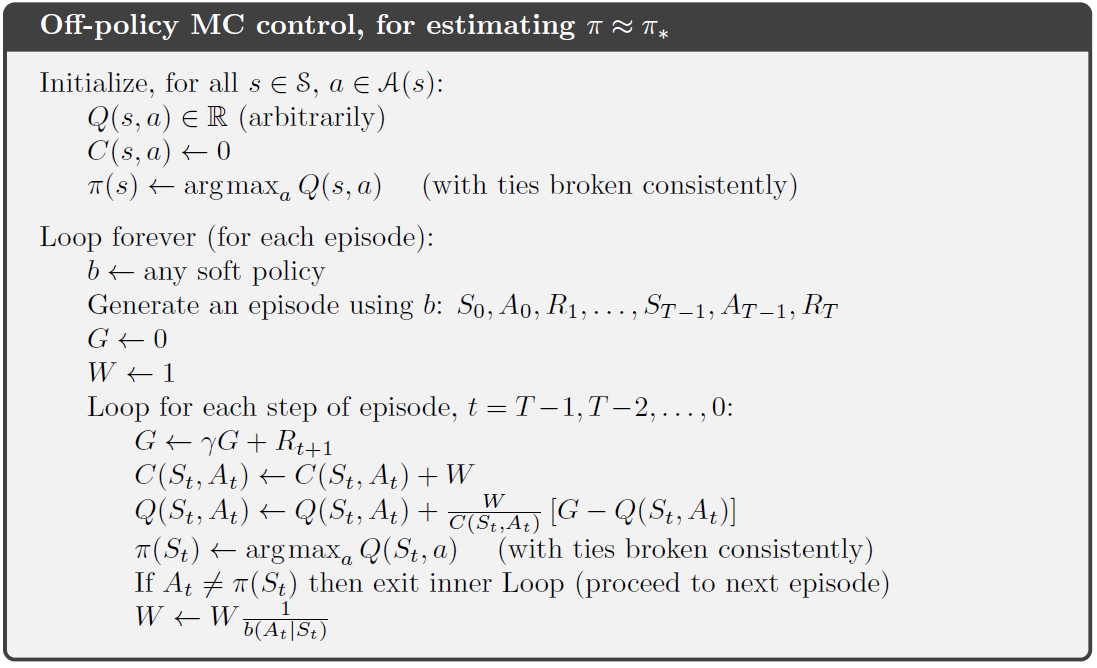
\includegraphics[width = 0.8 \textwidth]{alg_4.6.png}
\end{figure}

\end{exercise}

% --------------------------------------------------------------------------------

\begin{solution}

Converting (5.10) into action-values we obtain

\begin{align*}
  Q(s,a) \doteq \frac{\sum_{t \in \mathcal{T}(s,a)}\left(
  (1 - \gamma)\sum_{h=t+1}^{T(t) - 1} \gamma^{h - t - 1}\rho_{t:h-1}\bar{G}_{t:h} + 
  \gamma^{T(t) - t - 1} \rho_{t:T(t)-1}\bar{G}_{t:T(t)}\right)}
  {\sum_{t \in \mathcal{T}(s,a)}\left(
  (1 - \gamma)\sum_{h=t+1}^{T(t) - 1} \gamma^{h - t - 1}\rho_{t:h-1} + 
  \gamma^{T(t) - t - 1} \rho_{t:T(t)-1}\right)}
\end{align*}

If we define

\begin{align*}
  W_{t,h} &\doteq \begin{cases}
    (1 - \gamma)\gamma^{h - t - 1}\rho_{t:h-1}, & h < T(t) \\
    \gamma^{T(t) - t - 1}\rho_{t:T(t) - 1}, & h = T(t)
  \end{cases}
\end{align*}

we can rewrite the sum in a form, where we can use incremental implementation:

\begin{align*}
  Q(s,a) = \frac{\sum_{t \in \mathcal{T}(s,a)}\sum_{h=t+1}^{T(t)}W_{t,h}\bar{G}_{t:h}}
  {\sum_{t \in \mathcal{T}(s,a)}\sum_{h=t+1}^{T(t)}W_{t,h}}
\end{align*}
\begin{algorithm}
    \caption{Off-policy MC control, for estimating $\pi \approx \pi_*$}
    \begin{algorithmic}[1]
      \State Initialize $Q(s,a) \in \R$ arbitrarily for all $s \in \mathcal{S}, a \in \mathcal{A}(s)$
      \State Initialize $C(s,a) \leftarrow 0$
      \While{True (for each episode)}
        \State $b \leftarrow$ any soft policy
        \State Generate an episode following $b: S_0,A_0,R_1,\dots,S_{T-1},A_{T-1},R_T$
        \State $W \leftarrow $ array with length $T$, initialized with ones
        \For{$t = T-1,\dots,0$}
          \If{NOT $(S_t,A_t)$ appears in $(S_0,A_0),\dots,(S_{t-1},A_{t-1})$}
          \State $\rho \leftarrow 1$
          \State $G \leftarrow 0$
            \For{$h = t+1,\dots,T$}
              \State $G \leftarrow G + R_h$
              \State $\rho \leftarrow \rho \cdot \frac{\pi(A_{h-1}|S_{h-1})}{b(A_{h-1}|S_{h-1})}$
              \If{$h < T$}
                \State $C(S_t,A_t) \leftarrow C(S_t,A_t) + (1-\gamma)\gamma^{h - t - 1}\rho$
                \State $Q(S_t,A_t) \leftarrow Q(S_t,A_t) + 
                \frac{(1-\gamma)\gamma^{h - t - 1}\rho}{C(S_t,A_t)}(G - Q(S_t,A_t))$
              \Else
                \State $C(S_t,A_t) \leftarrow C(S_t,A_t) + \gamma^{T - t - 1}\rho$
                \State $Q(S_t,A_t) \leftarrow Q(S_t,A_t) + 
                \frac{\gamma^{T - t - 1}\rho}{C(S_t,A_t)}(G - Q(S_t,A_t))$
              \EndIf
            \EndFor
            \EndIf
        \EndFor
      \EndWhile
    \end{algorithmic}
\end{algorithm}

\FloatBarrier

\end{solution}

% --------------------------------------------------------------------------------
